\documentclass{beamer}
\usetheme{Singapore}
\usepackage[utf8]{inputenc}
\usecolortheme{crane}
\usepackage{graphicx}
\usepackage{iwona}
\usepackage{standalone}
\usepackage{tikz}
\usetikzlibrary{arrows}
\usetikzlibrary{decorations.markings}
\usetikzlibrary{calc}
\usetikzlibrary{shapes,snakes}
\usepackage{amsmath}
\usepackage{amsfonts}
\usepackage{amsthm}
\usepackage{mathtools}
\usepackage{tcolorbox}
\usepackage{hyperref}


\definecolor{lightblue}{RGB}{124,190,255}
\definecolor{darkgreen}{RGB}{24,145,0}

\beamertemplatenavigationsymbolsempty
\setbeamerfont{caption}{size=\tiny}
\setbeamertemplate{itemize items}{\textcolor{orange!50!yellow}{\textbullet}}
\setbeamertemplate{enumerate items}[square]
\setbeamercolor{item projected}{bg=orange!50!yellow}



\title
{A Brief Introduction to Markov Chains}
\author{Geraint Palmer}
\date{PGR Seminar 9/12/2015}
\titlegraphic{
\includegraphics[width=1.5cm]{cflogo}}



\begin{document}

\frame{\titlepage}

\begin{frame}
  \begin{enumerate}
    \vfill\item Discrete Time Markov Chains
    \begin{itemize}
      \vfill\item Steady-State Probabilities
      \vfill\item Higher Order Markov Chains
    \end{itemize}
    \vfill\item Absorbing Markov Chains
    \begin{itemize}
      \vfill\item Snakes \& Ladders
    \end{itemize}
    \vfill\item Continuous Time Markov Chains
    \begin{itemize}
      \vfill\item A Simple Queue
    \end{itemize}
  \end{enumerate}
\end{frame}



\begin{frame}
\begin{figure}
  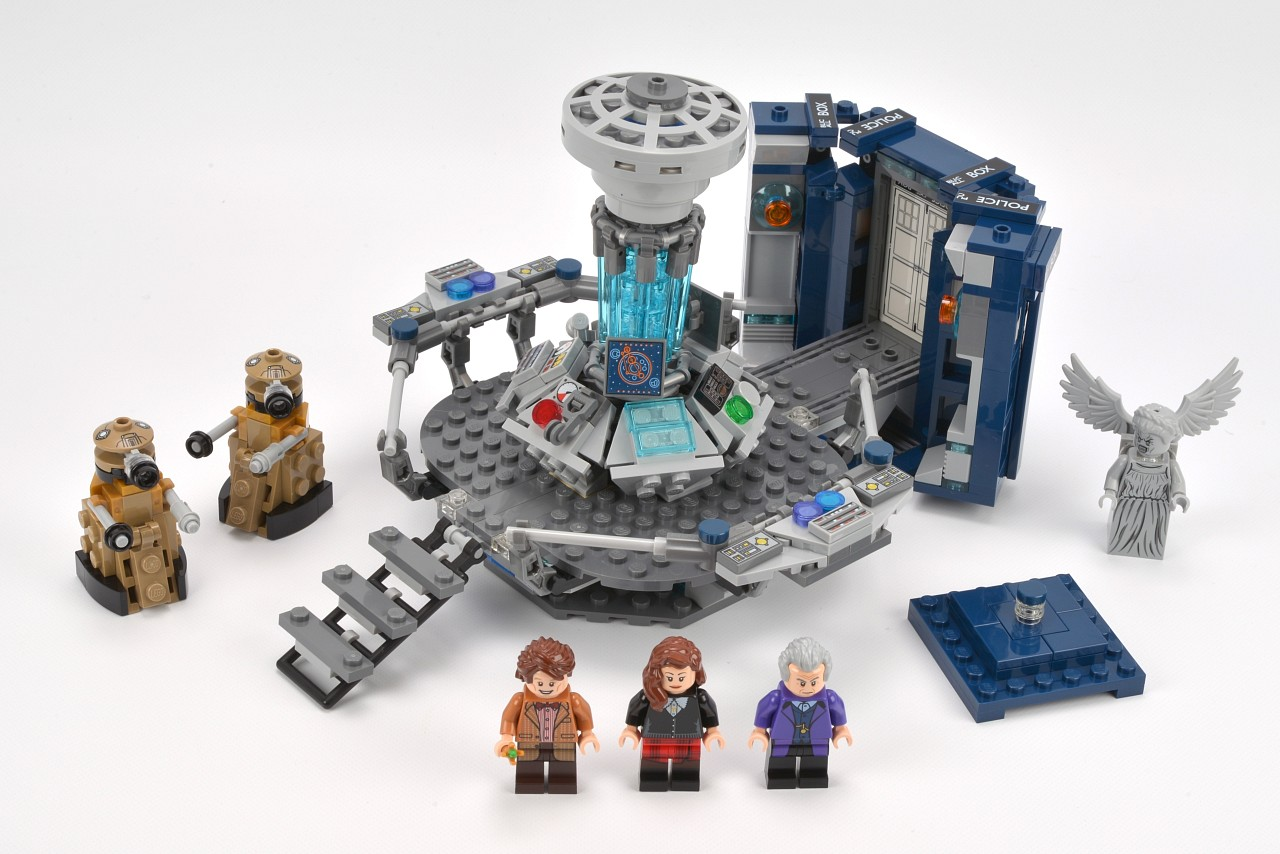
\includegraphics[width=\textwidth]{lego_drwho}
  \caption{from Flickr \href{https://www.flickr.com/photos/brickset/}{\textcolor{blue}{brickset}}}
\end{figure}
\end{frame}



\begin{frame}
\frametitle{Andrei Andreyevich Markov}
\begin{figure}
  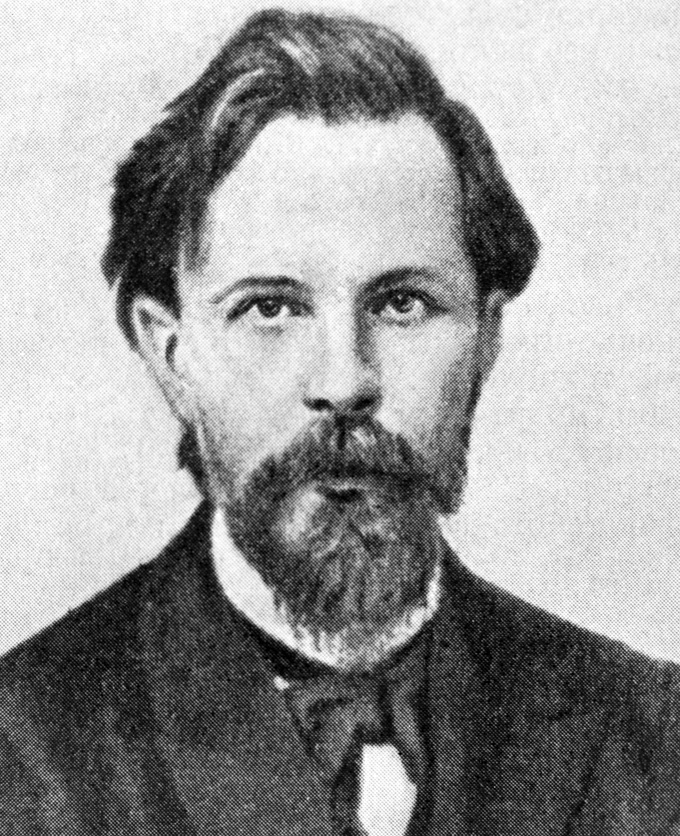
\includegraphics[width=0.5\textwidth]{andreimarkovmathematician}
  \caption{Markov chain pioneer.}
\end{figure}
\end{frame}



\begin{frame}
\frametitle{What is a Markov Chain?}
\begin{figure}
  \includestandalone[width=\textwidth]{MC_ABC}
\end{figure}
\end{frame}



\begin{frame}
\huge{
\begin{equation*}
 P =  \left( \begin{array}{ccc}
0.5 & 0.2 & 0.3 \\
0.8 & 0.1 & 0.1 \\
0.2 & 0.6 & 0.2 \end{array} \right)
\end{equation*}
}
\end{frame}



\begin{frame}
\begin{figure}
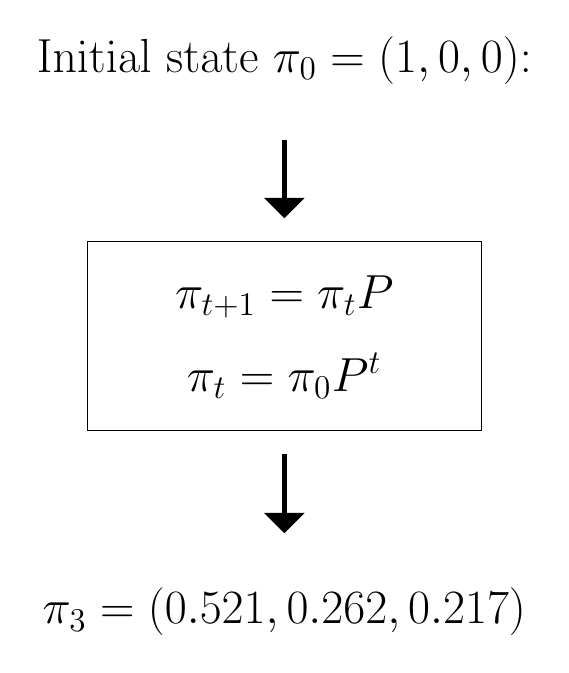
\begin{tikzpicture}
\node at (0, 6) {\LARGE Initial state $\pi_0 = (1, 0, 0)$:};

\draw[ultra thick, -triangle 90] (0, 5) -- (0, 4);
\draw[ultra thick, -triangle 90] (0, 1) -- (0, 0);

\draw (-2.5, 1.3) rectangle (2.5, 3.7);
\node at (0, 3.0) {\LARGE $\pi_{t+1} = \pi_t P$};
\node at (0, 2.0) {\LARGE $\pi_{t} = \pi_0 P^t$};

\node at (0, -1) {\LARGE $\pi_3 = (0.521, 0.262, 0.217)$};
\end{tikzpicture}
\end{figure}
\end{frame}




\begin{frame}
\begin{figure}
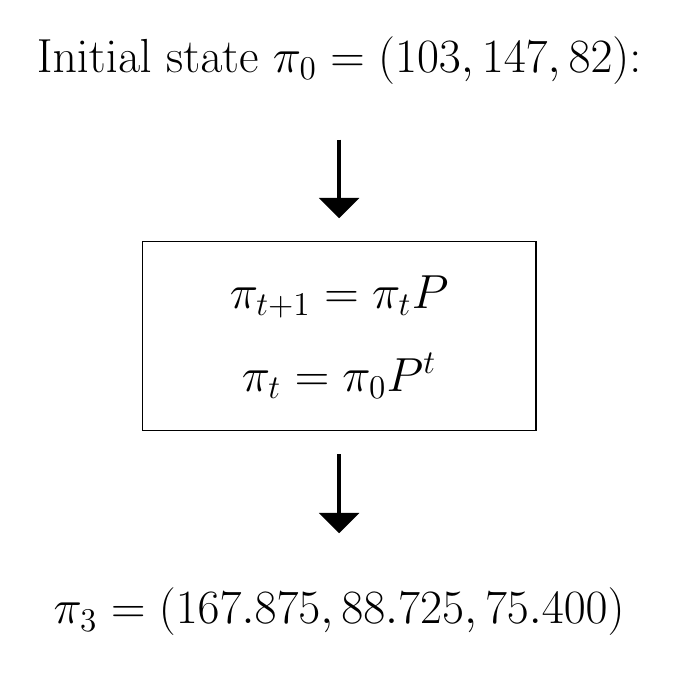
\begin{tikzpicture}
\node at (0, 6) {\LARGE Initial state $\pi_0 = (103, 147, 82)$:};

\draw[ultra thick, -triangle 90] (0, 5) -- (0, 4);
\draw[ultra thick, -triangle 90] (0, 1) -- (0, 0);

\draw (-2.5, 1.3) rectangle (2.5, 3.7);
\node at (0, 3.0) {\LARGE $\pi_{t+1} = \pi_t P$};
\node at (0, 2.0) {\LARGE $\pi_{t} = \pi_0 P^t$};

\node at (0, -1) {\LARGE $\pi_3 = (167.875, 88.725, 75.400)$};
\end{tikzpicture}
\end{figure}
\end{frame}




\begin{frame}
\begin{figure}
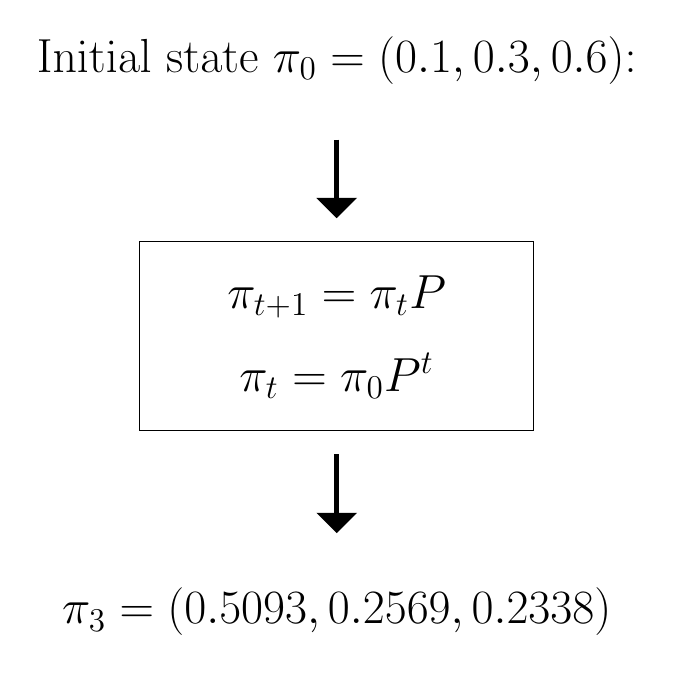
\begin{tikzpicture}
\node at (0, 6) {\LARGE Initial state $\pi_0 = (0.1, 0.3, 0.6)$:};

\draw[ultra thick, -triangle 90] (0, 5) -- (0, 4);
\draw[ultra thick, -triangle 90] (0, 1) -- (0, 0);

\draw (-2.5, 1.3) rectangle (2.5, 3.7);
\node at (0, 3.0) {\LARGE $\pi_{t+1} = \pi_t P$};
\node at (0, 2.0) {\LARGE $\pi_{t} = \pi_0 P^t$};

\node at (0, -1) {\LARGE $\pi_3 = (0.5093, 0.2569, 0.2338)$};
\end{tikzpicture}
\end{figure}
\end{frame}



\begin{frame}
\frametitle{Steady-State Probabilities}
\LARGE \begin{equation*}
\pi = \pi P
\end{equation*}
\begin{equation*}
\Sigma \pi = 1
\end{equation*}
\begin{figure}
  \includestandalone[width=0.75\textwidth]{steadystates}
\end{figure}
\end{frame}



\begin{frame}
\frametitle{The Markov Property}
\begin{figure}
  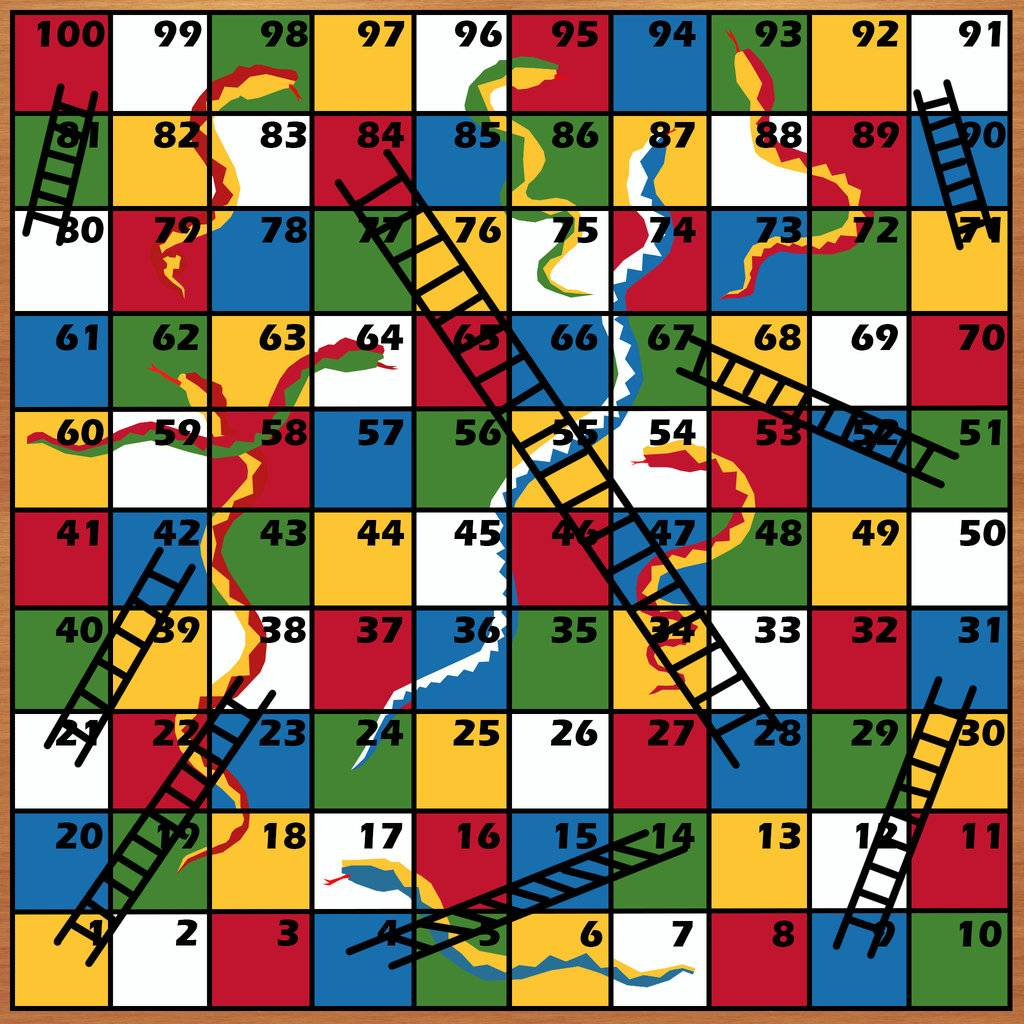
\includegraphics[width=0.65\textwidth]{snakes_and_ladders}
\end{figure}
\end{frame}



\begin{frame}
\frametitle{Higher Order Markov Chains}
\begin{figure}
  \includestandalone[width=0.65\textwidth]{secondorderMC}
\end{figure}
\end{frame}

\begin{frame}
\frametitle{Higher Order Markov Chains}
\begin{figure}
  \includestandalone[width=0.65\textwidth]{secondorderMCdetail}
\end{figure}
\end{frame}



\begin{frame}
\begin{figure}
  \includestandalone[width=\textwidth]{memorydepthwords1}
\end{figure}
\end{frame}
\begin{frame}
\begin{figure}
  \includestandalone[width=\textwidth]{memorydepthwords2}
\end{figure}
\end{frame}
\begin{frame}
\begin{figure}
  \includestandalone[width=\textwidth]{memorydepthwords3}
\end{figure}
\end{frame}



\begin{frame}
\frametitle{Generating Music with Markov Chains}
\url{https://www.youtube.com/watch?v=qOZ2Q-Ls48U}
\end{frame}



\begin{frame}
\frametitle{Classification of States}
\begin{figure}
  \includestandalone[width=\textwidth]{classifystates}
\end{figure}
\end{frame}


\begin{frame}
\frametitle{Absorbing Markov Chains}

\begin{tcolorbox}[colback=orange!25!yellow!25,colframe=orange!50!yellow,title=\textit{Probability of Absorption},coltitle=black]

\begin{equation*}
\mathbb{P}\left(\text{absorption in $t$ steps from } s\right) = P^{t}_{(s,a)}
\end{equation*}

\begin{equation*}
\lim_{t\to\infty}P^{t}_{(s,a)} \rightarrow 1
\end{equation*}
\end{tcolorbox}
\pause

\begin{tcolorbox}[colback=orange!25!yellow!25,colframe=orange!50!yellow,title=\textit{Mean Steps to Absorption},coltitle=black]

\begin{equation*}
P = \left(\begin{array}{cc}Q & R\\
\textbf{0} & 1\end{array}\right)
\end{equation*}

\begin{equation*}
\mathbb{E}\left[\text{steps to absorption from } s\right] = {\left(\mathbb{I} - Q\right)^{-1}}_{(s)}
\end{equation*}
\end{tcolorbox}

\end{frame}




\begin{frame}
\begin{figure}
  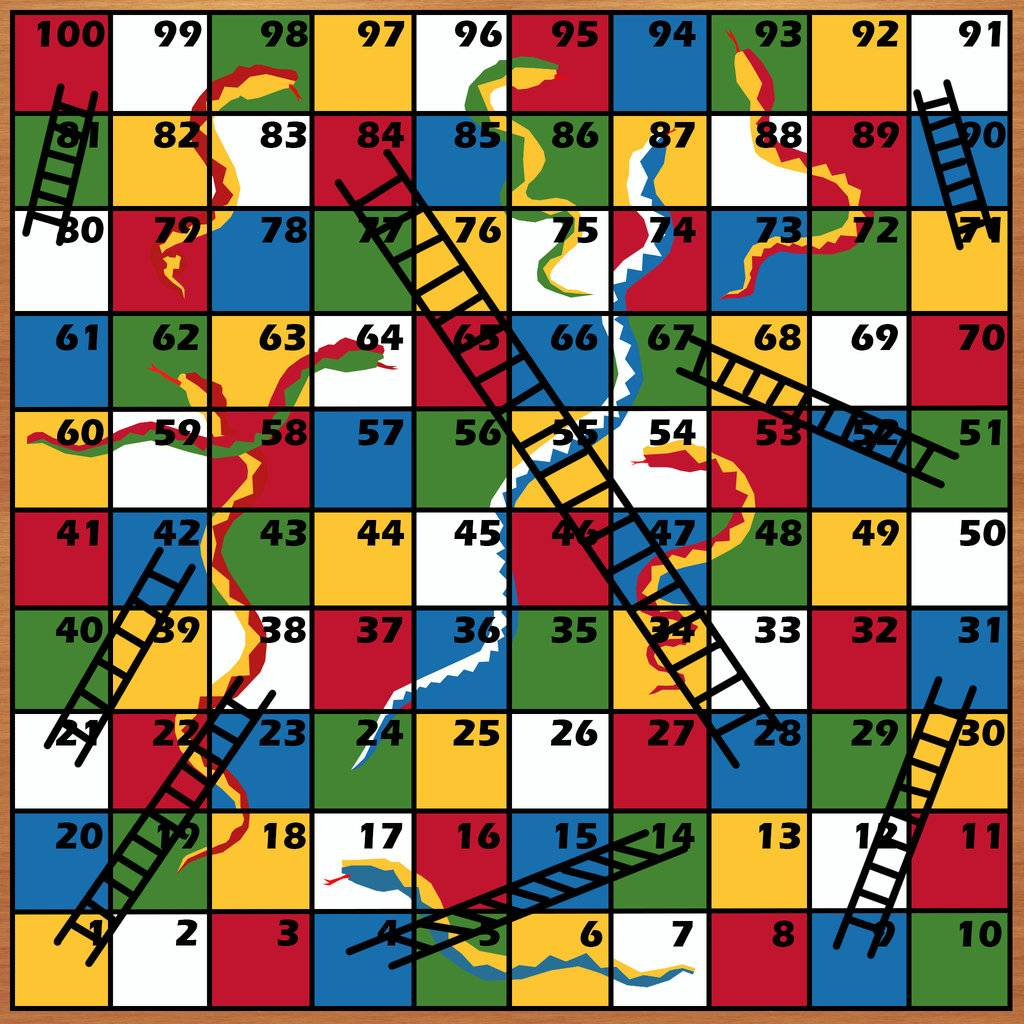
\includegraphics[width=0.65\textwidth]{snakes_and_ladders}
\end{figure}
\end{frame}

\begin{frame}
\begin{figure}
  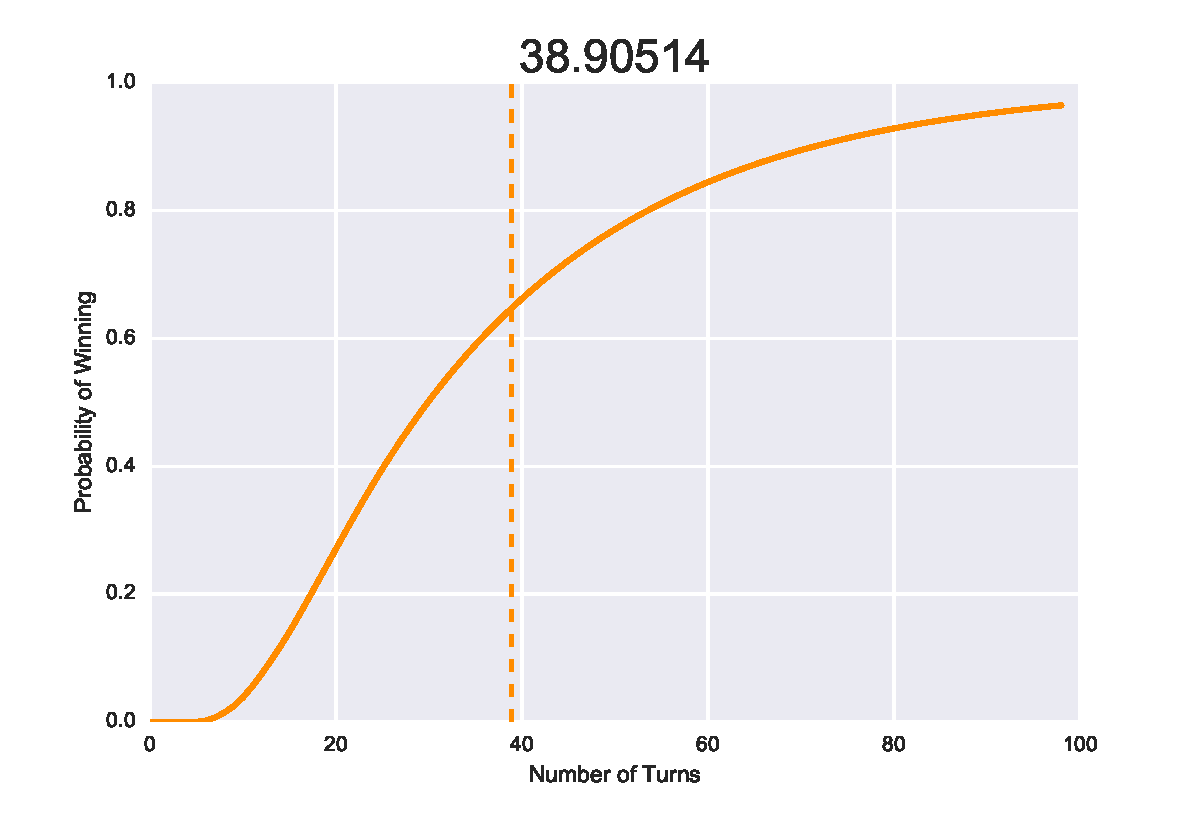
\includegraphics[width=0.9\textwidth]{snakesladdersabs}
\end{figure}
\end{frame}



\begin{frame}
\frametitle{Continuous-Time Markov Chains}
\begin{figure}
  \includestandalone[width=0.9\textwidth]{MC_ABC_continuous}
\end{figure}
\end{frame}

\begin{frame}
\huge{
\begin{equation*}
 Q =  \left( \begin{array}{ccc}
-13.8 & 7.5 & 6.3 \\
4.0 & -9.8 & 5.8 \\
11.2 & 2.9 & -14.1 \end{array} \right)
\end{equation*}
}
\end{frame}



\begin{frame}
\begin{center}
\begin{tabular}{p{3cm}|p{5.5cm}}
\Large Discrete & \Large Continuous \\[5ex]
\Large $ \pi_t = \pi_0P^{t} $ & \Large $ \pi_t = \pi_0\left(\mathbb{I} + \sum_{k=1}^{\infty}\frac{Q^kt^k}{k!}\right) $ \\[5ex]
\Large $ \pi = \pi P $ & \Large $ 0 = \pi Q $ \\[5ex]
\end{tabular}
\end{center}
\end{frame}


\begin{frame}
\frametitle{The Exponential Distribution}
\begin{center}
$f(x) = \lambda e^{-\lambda x}$
\begin{figure}
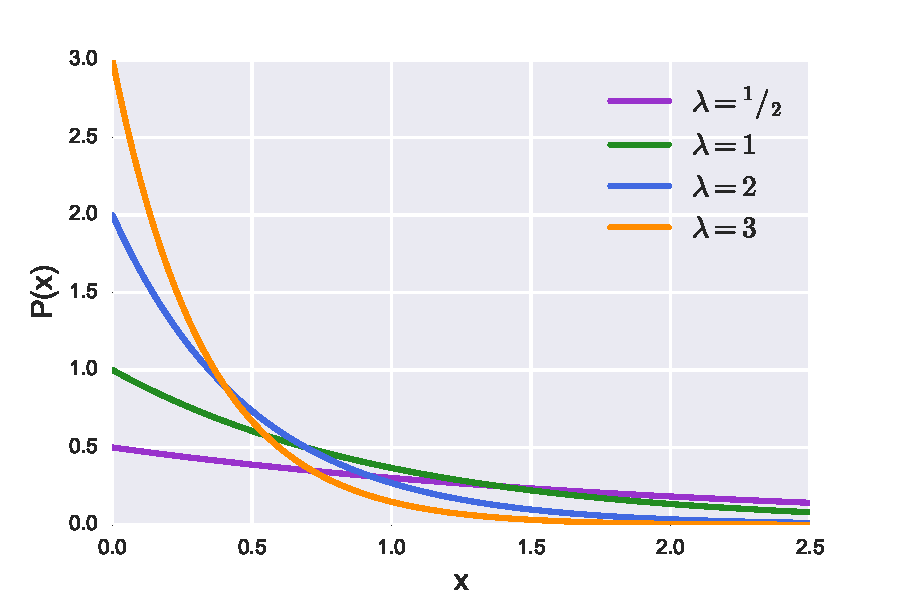
\includegraphics[width=0.75\textwidth]{expon_dist}
\end{figure}
$\mathbb{P}\left(T > s + t \nonscript\; | \nonscript\; T > t\right) = \mathbb{P}\left(T > s\right)$
\end{center}
\end{frame}


\begin{frame}
\frametitle{Modelling a Queue}
\begin{figure}
  \includestandalone[width=\textwidth]{mm12Q}
\end{figure}

\begin{tcolorbox}[colback=orange!25!yellow!25,colframe=orange!50!yellow]
\begin{center}
Arrivals $\sim$ Poisson($\lambda$)\\
Service time $\sim$ Exponential($\mu$)
\end{center}
\end{tcolorbox}
\end{frame}




\begin{frame}
\begin{figure}
  \includestandalone[width=\textwidth]{queueMC}
\end{figure}
\end{frame}


\begin{frame}
\begin{equation*}
  Q = \left(\begin{array}{cccc}
  -\lambda & \lambda & 0 & 0 \\
  \mu & -(\lambda+\mu) & \lambda & 0 \\
  0 & \mu & -(\lambda+\mu) & \lambda \\
  0 & 0 & \mu & -\mu\end{array}\right)
\end{equation*}
\pause
\begin{align*}
\pi_0 &= \frac{\mu^3}{\lambda^3 + \lambda^2\mu + \lambda\mu^2 + \mu^3}\\
\pi_1 &= \frac{\lambda\mu^2}{\lambda^3 + \lambda^2\mu + \lambda\mu^2 + \mu^3}\\
\pi_2 &= \frac{\lambda^2\mu}{\lambda^3 + \lambda^2\mu + \lambda\mu^2 + \mu^3}\\
\pi_3 &= \frac{\lambda^3}{\lambda^3 + \lambda^2\mu + \lambda\mu^2 + \mu^3}
\end{align*}
\end{frame}



\begin{frame}
\begin{center}
\huge Thank You!
\end{center}
\end{frame}

\end{document}
